% !TEX encoding = UTF-8
% !TEX TS-program = pdflatex
% !TEX root = ../tesi.tex

%**************************************************************
\chapter{Integrazione in SyncTrace}
\label{cap:integrazione-synctrace}
\intro{In questo capitolo viene mostrata l'integrazione dello smart contract con l'applicazione mobile e la web application di SyncTrace.}\\

\section{Applicazione android}
\begin{figure}[!htb]
   \begin{minipage}{0.48\textwidth}
     \centering
     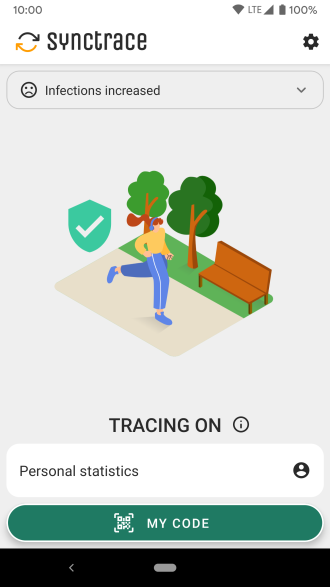
\includegraphics[width=0.65\textwidth]{./immagini/appnormal}
     \caption{Schermata principale SyncTrace senza rischio contagio}
   \end{minipage}\hfill
   \begin{minipage}{0.48\textwidth}
     \centering
     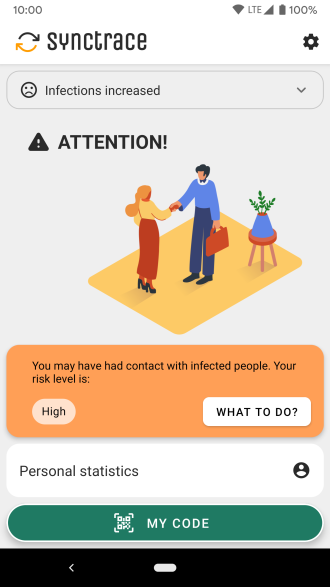
\includegraphics[width=0.65\textwidth]{./immagini/appinfection}
     \caption{Schermata principale SyncTrace con rischio contagio}
   \end{minipage}
\end{figure}
\FloatBarrier
\subsection{Obiettivo}
L'obiettivo dell'integrazione con l'applicazione è implementare una classe che gestisca il contratto e tutte le operazioni legate alla \textit{blockchain}, come visto in fase di progettazione. In particolare è necessario avere a disposizione:
\begin{itemize}
	\item{Credenziali per ogni utente da creare al primo avvio dell'app;}
	\item{Trasferimento di \textit{Ether} a ogni utente, con ricarica all'esaurimento;}
	\item{Gestione delle funzioni dello \textit{smart contract} richieste dall'applicazione, come l'aggiunta dei contatti.}
\end{itemize}

\subsection{Generazione classe Tracing.java}
Per potere utilizzare lo \textit{smart contract}, bisogna generare una classe Java a partire dal contratto, sfruttando \textit{web3j}. La classe generata renderà disponibili i metodi dello \textit{smart contract}, oltre a funzioni per effettuare il \textit{deployment} e caricare un contratto.\\\\
La prima cosa da fare è scaricare \textit{web3j} dalla repo su \href{https://github.com/web3j/web3j/releases}{Github} ed estrarre il file zip scaricato con il comando:
\begin{lstlisting}[numbers=none]
	unzip web3j-<version>.zip
\end{lstlisting}
Sempre da terminale, si può avviare web3j in questo modo:
\begin{lstlisting}[numbers=none]
	web3j-<version>/bin/web3j
\end{lstlisting}
A questo punto è possibile creare i file .abi e .bin dello smart contract con il comando: 
\begin{lstlisting}[numbers=none]
	solcjs ./Tracing.sol --bin --abi --optimize -o ./ 
\end{lstlisting}
A partire dai file .bin e .abi si può finalmente generare la classe java:
\begin{lstlisting}[numbers=none]
	web3j solidity generate -b ./Tracing.bin -a ./Tracing.abi -o ./ -p GeneratedClasses 
\end{lstlisting}
In questo modo nella directory GeneratedClasses si troverà la classe Tracing.java, da inserire nel progetto di android per permettere l'integrazione dell'app con la blockchain.
L'ultimo passaggio da effettuare per interagire con il contract è includere nel file build.gradle del progetto la dipendenza con la libreria web3j, inserendo la seguente riga:
\begin{lstlisting}[numbers=none]
	implementation'org.web3j:core:<version>' 
\end{lstlisting}

\subsection{Implementazione}
Oltre alla classe \textit{Tracing.java}, generata da \textit{web3j}, è necessario implementare una classe che si occupi di configurare e gestire le operazioni in \textit{blockchain}.
Nel progetto SyncTrace è stata creata la classe \textit{BlockchainManager} per questo scopo, scritta in linguaggio Kotlin come il resto dell'applicazione.
Per configurare correttamente il collegamento con lo \textit{smart contract} sono necessarie le seguenti variabili:
\begin{lstlisting}[language = Kotlin]
    private val GAS_LIMIT = BigInteger.valueOf(GAS_LIMIT)
    private val GAS_PRICE = BigInteger.valueOf(GAS_PRICE)
    private const val PRIVATE_KEY = YOUR_PRIVATE_KEY
    private const val CONTRACT_ADDRESS = ADDRESS
    private const val CREDENTIALS = "bc_credentials"
    private const val TRANSACTION_CREDENTIALS = "bc_transaction_credentials"
    private val web3j = Web3j.build(HttpService(
        "https://ropsten.infura.io/v3/YOUR_INFURA_ID"
    ))
\end{lstlisting}
\mbox{\\}

\textit{GAS\_LIMIT} e \textit{GAS\_PRICE} sono i valori relativi al gas in \textit{Ethereum} e devono essere passati nelle funzioni che richiedono una transazione.\\\\
La variabile \textit{PRIVATE\_KEY} è la chiave privata dell'account \emph{\gls{Metamask}}\glsfirstoccur che finanzia l'applicazione.\\\\
\textit{CONTRACT\_ADDRESS} è l'indirizzo del contratto nella \textit{blockchain}. È possibile effettuare il \textit{deployment} anche tramite \textit{web3j} e ottenere l'\textit{address} del contratto da utilizzare.\\\\
\textit{CREDENTIALS} e \textit{TRANSACTION\_CREDENTIALS} rappresentano le keyword utilizzate per salvare le credenziali nelle \textit{shared preferences} di android. Vengono create al primo avvio dell'app e salvate per essere utilizzate nel chiamare le funzioni dello \textit{smart contract}.\\\\ 
\textit{web3j} è un'istanza utilizzata per fornire un client eseguito tramite il provider Infura.\\\\

\newpage
Nella classe sono disponibili alcune funzioni di utilità utilizzate dai metodi che verranno successivamente descritti:
\begin{lstlisting}[language = Kotlin]

/*
Controlla se le credenziali siano gia' state salvate nelle shared preferences
*/
private fun areCredentialsPresent(context: Context): Boolean


/*
Ritorna le credenziali dell'utente dalle shared preferences
*/
private fun getCredentials(context: Context): Credentials

/*
Ritorna le credenziali dell'admin dalle shared preferences
*/
private fun getTransactionCredentials(context: Context): Credentials

/*
Salva le credenziali nelle shared preferences
*/
private fun setCredentials(context: Context, credentials: Credentials,
                               transactionCredentials: Credentials)

/*
Ritorna un'istanza del contratto
*/
private fun loadContract(context: Context, credentials: Credentials = getCredentials(context)): TracingContract

/*
Effettua una transazione dall'account admin all'account utente
*/
private fun sendFunds(context: Context, amount: Double,
                          credentials: Credentials = getCredentials(context),
                          transactionCredentials: Credentials = getTransactionCredentials(context))
\end{lstlisting} 

\newpage
Al primo avvio dell'applicazione bisogna creare delle credenziali per il nuovo account, effettuare una transazione verso questo account, caricare il contratto \textit{Tracing} e infine aggiungere l'utente in \textit{blockchain} tramite la funzione \textit{addPerson} dello \textit{smart contract}. La funzione \textit{registerPersonIfFirstTime} si occupa di tutto ciò
\begin{lstlisting}[language = Kotlin]
    fun registerPersonIfFirstTime(context: Context) {
        if (!areCredentialsPresent(context)) {
            val transactionCredentials = Credentials.create(PRIVATE_KEY)
            // create new private/public key pair
            val keys = Keys.createEcKeyPair()
            val uuid = User.getUuid(context)
            val wallet = Wallet.createLight(uuid, keys)
            val credentials = Credentials.create(Wallet.decrypt(uuid, wallet))

            sendFunds(context, 0.2, credentials, transactionCredentials)

            try {
                val tracingContract = loadContract(context, credentials)
                tracingContract.addPerson(uuid, credentials.address).sendAsync().get()
            } catch (e: Exception) {
                Log.e(TAG, "Cannot add person", e)
                return
            }

            setCredentials(context, credentials, transactionCredentials)
            Log.i(TAG, "Created credentials and registered person")
        }
    }
\end{lstlisting}

\newpage
Infine la classe \textit{BlockchainManager} deve fornire una funzione per ogni metodo del contratto che viene utilizzato nell'applicazione, come per il metodo \textit{addContact} che aggiunge un contatto in \textit{blockchain} quando rilevato dal bluetooth.

\mbox{\\}
\begin{lstlisting}[language = Kotlin]
    fun addContact(context: Context, myUuid: String, contactUuid: String, contactIndex: Double) {
        try {
            val tracingContract = loadContract(context)
            tracingContract.addContact(myUuid, contactUuid, BigInteger.valueOf(contactIndex.toLong()))
                .sendAsync().get()

            val ethGetBalance =
                web3j.ethGetBalance(CONTRACT_ADDRESS, DefaultBlockParameterName.LATEST).sendAsync().get()
            val wei = ethGetBalance!!.balance
            if (wei.compareTo(BigInteger.valueOf(100000000000000000L)) == -1) {
                sendFunds(context, 0.1)
            }
        } catch (e: Exception) {
            Log.e(TAG, "Cannot add contact to blockchain", e)
        }
    }
\end{lstlisting}
\mbox{\\}

È importante soffermarsi sulla funzione \textit{addContact} per alcune considerazioni:
\begin{itemize}
	\item{La chiamata al metodo \textit{addContact} deve essere asincrona, per permettere all'applicazione di continuare l'esecuzione senza interruzioni. La transazione in \textit{Ethereum} non è immediata ed è opportuno che in questo lasso di tempo l'applicazione non si interrompa;}
	\item{Dopo l'esecuzione della transazione viene controllato il \textit{balance} dell'account e, se risulta inferiore a una certa soglia, viene ricaricato;}
	\item{Possono essere sollevate eccezioni nel caso in cui la transazione non vada a buon fine; per questo è importare gestirle correttamente per evitare crash dell'applicazione.}
\end{itemize}


\section{Web application}
\subsection{Obiettivo}
La web application di SyncTrace è utilizzata dal personale sanitario per avere un'interfaccia di gestione con dei privilegi speciali. Tra questi spicca l'inserimento di una persona infetta dopo il risultato positivo di un tampone. Lo \textit{smart contract} ha un metodo che permette di farlo e l'obiettivo di questa sezione è mostrare l'interazione con la \textit{blockchain} in ambiente web.
\newpage
\subsection{Implementazione}
La web app ha la seguente pagina dedicata all'inserimento di un infetto nel sistema 
\begin{figure}[h]
\caption{Inserimento infetti da web application}
\centering
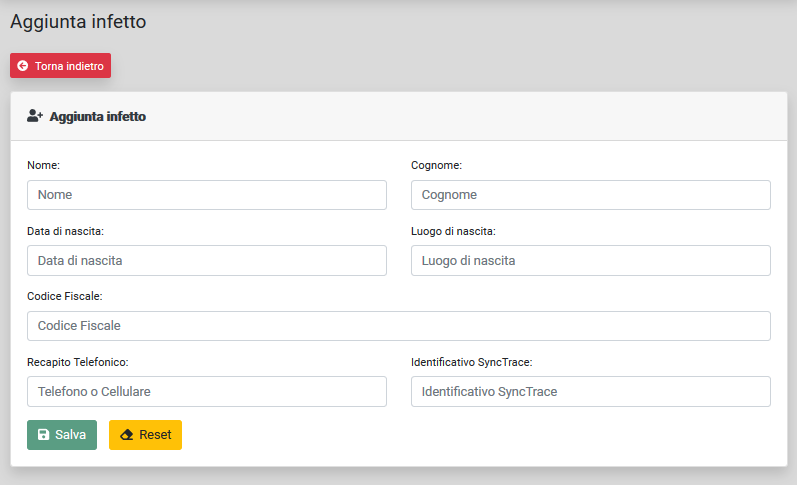
\includegraphics[width=1.0\textwidth]{./immagini/webapp_infected}
\end{figure}
\FloatBarrier

Al momento del salvataggio dei dati presenti nel form, deve essere effettuata una chiamata al metodo \textit{setInfected} dello \textit{smart contract}.
Come mostrato nell'implementazione dello \textit{smart contract}, solo l'\textit{address} dell'admin può chiamare questa funzione. In caso contrario viene lanciata un'eccezione e l'inserimento viene rigettato. Così facendo c'è la certezza che nessuno possa modificare scorrettamente i dati in \textit{blockchain}.\\\\

Per implementare quanto descritto si sfrutta la libreria \textit{web3js}, con i seguenti import:

\begin{lstlisting}
import Web3 from 'web3';
import * as eth from 'ethereumjs-tx';
const Tx = eth.Transaction;
\end{lstlisting}

Le variabili per configurare il contratto e completare correttamente le transazioni in \textit{Ethereum} sono le seguenti:
\begin{lstlisting}
    private web3 = new Web3(new Web3.providers.HttpProvider('https://ropsten.infura.io/v3/YOUR_INFURA_ID'));
    private adminAddress = 'ADMIN_ADDRESS';
    private privKey = environment.BC_PRIVATE_KEY;
    private contractAddress = ''CONTRACT_ADDRESS;
    private abiContract = 'CONTRACT_ABI'
    private myContract = new this.web3.eth.Contract(JSON.parse(this.abiContract), this.contractAddress);
\end{lstlisting}

\textit{web3} è un'istanza utilizzata per fornire un client eseguito tramite il provider Infura.\\
\textit{adminAddress} è l'indirizzo di chi ha effettuato il \textit{deployment}, l'unico con l'autorità per chiamare la funzione \textit{setInfected}.\\
\textit{privKey} rappresenta la chiave privata dell'admin.\\
\textit{contractAddress} è l'indirizzo in cui risiede il contratto nella \textit{blockchain}.\\
\textit{abiContract} è il contratto in formato abi, necessario per creare l'instanza del contratto \textit{myContract}, insieme all'indirizzo del contratto.\\

Per inviare la transazione in \textit{Ethereum} è presente la seguente funzione, che prende in input i dati e effettua la transazione grazie alla funzione di web3js:

\begin{lstlisting}
  sendSigned(txData, cb) {
    const privateKey = Buffer.from(this.privKey, 'hex');
    const transaction = new Tx(txData, {chain: 'ropsten'});
    transaction.sign(privateKey);
    const serializedTx = transaction.serialize().toString('hex');
    this.web3.eth.sendSignedTransaction('0x' + serializedTx, cb);
  }
\end{lstlisting}

Infine, le seguenti righe di codice si occupano di creare i dati della transazione chiamando il metodo \textit{setInfected} per poi inviare la transazione sfruttando la funzione \textit{sendSigned}:
\begin{lstlisting}

  createInfected(infected: Infected) {

    const myData = this.myContract.methods.setInfected( infected.infected_id, true).encodeABI();

    this.web3.eth.getTransactionCount(this.addressFrom).then(txCount => {

      const txData = {
        nonce: this.web3.utils.toHex(txCount),
        gasLimit: this.web3.utils.toHex(GAS_LIMIT),
        gasPrice: this.web3.utils.toHex(GAS_PRICE),
        to: this.contractAddress,
        from: this.adminAddress,
        value: this.web3.utils.toHex(this.web3.utils.toWei('0', 'wei')),
        data: myData
      };

      this.sendSigned(txData, (err, result) => {
        if (err) {
           return console.log('error', err);
        }
        console.log('sent', result);
      });
  }
\end{lstlisting}

Dopo questa serie di operazioni, il codice identificativo della persona inserita tramite interfaccia web, viene segnalato come infetto in \textit{blockchain} e, dall'applicazione mobile, gli utenti che hanno registrato un contatto con l'identificativo segnalato verranno avvertiti di conseguenza.

